% SACRILEGE ENGINE - IEEE Conference Presentation
% LaTeX Beamer Presentation
% Compile with: pdflatex presentation.tex

\documentclass[aspectratio=169]{beamer}

% Theme
\usetheme{Madrid}
\usecolortheme{whale}
\setbeamertemplate{navigation symbols}{}
\setbeamertemplate{footline}[frame number]

% Packages
\usepackage{graphicx}
\usepackage{booktabs}
\usepackage{amsmath}
\usepackage{listings}
\usepackage{xcolor}
\usepackage{tikz}
\usetikzlibrary{shapes,arrows,positioning}

% Colors
\definecolor{ctblue}{RGB}{60,140,255}
\definecolor{torange}{RGB}{255,170,40}
\definecolor{accent}{RGB}{0,220,255}
\definecolor{darkbg}{RGB}{6,8,12}

% Code style
\lstset{
    basicstyle=\ttfamily\footnotesize,
    backgroundcolor=\color{darkbg!10},
    frame=single,
    breaklines=true
}

% Title
\title[Sacrilege Engine]{SACRILEGE ENGINE}
\subtitle{A Real-Time CS2 Demo Analysis System with Blame Attribution}
\author{Pl4yer-ONE}
\institute{mahadevan.rajeev27@gmail.com}
\date{January 2026}

\begin{document}

% Title Slide
\begin{frame}
\titlepage
\end{frame}

% Outline
\begin{frame}{Outline}
\tableofcontents
\end{frame}

% Section 1
\section{Introduction}

\begin{frame}{Problem Statement}
\begin{columns}
\column{0.5\textwidth}
\textbf{Traditional Tools}
\begin{itemize}
    \item[$\times$] Team-level stats only
    \item[$\times$] Post-match summaries
    \item[$\times$] "You died 15 times"
    \item[$\times$] Abstract K/D ratios
\end{itemize}

\column{0.5\textwidth}
\textbf{Sacrilege Engine}
\begin{itemize}
    \item[\checkmark] Individual death analysis
    \item[\checkmark] Real-time feedback
    \item[\checkmark] \textbf{Why} you died 15 times
    \item[\checkmark] Blame scores per death
\end{itemize}
\end{columns}

\vspace{1em}
\begin{alertblock}{Gap}
No tool assigns accountability to individual deaths with tactical reasoning.
\end{alertblock}
\end{frame}

% Section 2
\section{Methodology}

\begin{frame}{System Architecture}
\begin{center}
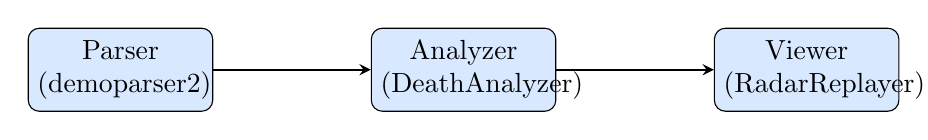
\begin{tikzpicture}[node distance=2cm, auto]
    \tikzstyle{block} = [rectangle, draw, fill=ctblue!20, text width=6em, text centered, rounded corners, minimum height=3em]
    \tikzstyle{arrow} = [thick,->,>=stealth]

    \node [block] (parser) {Parser\\(demoparser2)};
    \node [block, right=of parser] (analyzer) {Analyzer\\(DeathAnalyzer)};
    \node [block, right=of analyzer] (viewer) {Viewer\\(RadarReplayer)};

    \draw [arrow] (parser) -- (analyzer);
    \draw [arrow] (analyzer) -- (viewer);
\end{tikzpicture}
\end{center}

\begin{itemize}
    \item \textbf{Parser}: Extract kills, positions, utility from .dem files
    \item \textbf{Analyzer}: Classify mistakes, compute blame scores
    \item \textbf{Viewer}: Render radar with live statistics
\end{itemize}
\end{frame}

\begin{frame}{Mistake Classification System}
\begin{table}
\centering
\begin{tabular}{clp{6cm}}
\toprule
\textbf{Severity} & \textbf{Category} & \textbf{Description} \\
\midrule
5 & ISOLATED & Died alone, no support possible \\
5 & CROSSFIRE & Exposed to multiple angles \\
5 & SOLO\_PUSH & Pushed alone into enemy territory \\
4 & NO\_TRADE & Teammate close but didn't trade \\
4 & WIDE\_PEEK & Over-extended peek \\
3 & FLASHED & Killed while blinded \\
3 & OUTNUMBERED & Took unfavorable fight \\
2 & FIRST\_CONTACT & Entry death (acceptable) \\
1 & FAIR\_DUEL & Lost aim battle \\
1 & TRADED & At least got traded \\
\bottomrule
\end{tabular}
\caption{15 Tactical Mistake Categories}
\end{table}
\end{frame}

\begin{frame}{Blame Score Algorithm}
\begin{block}{Formula}
\[
\text{Blame Score} = (\text{Severity} \times 20) + \text{Modifiers}
\]
\end{block}

\textbf{Modifiers:}
\begin{itemize}
    \item Isolation (distance $>$ 1000 units): $+10$
    \item Multiple enemies ($\geq 3$): $-10$
    \item Was traded: $-15$
    \item Was flashed: $-5$
\end{itemize}

\begin{exampleblock}{Example}
Player isolated in crossfire:
\[
\text{Base} = 5 \times 20 = 100, \quad +10 \text{ (isolated)}, \quad -10 \text{ (3 enemies)}
\]
\[
\text{Final} = \min(100, \max(0, 100)) = \textbf{100\% blame}
\]
\end{exampleblock}
\end{frame}

\begin{frame}{Performance Grading}
\begin{block}{Performance Score Formula}
\[
\text{Score} = (\text{K/D} \times 40) - (\text{Avg Blame} \times 0.4) + 20
\]
\end{block}

\begin{table}
\centering
\begin{tabular}{ccc}
\toprule
\textbf{Grade} & \textbf{Threshold} & \textbf{Meaning} \\
\midrule
\textcolor{yellow!80!black}{\textbf{S}} & $\geq 80$ & Elite \\
\textcolor{green}{\textbf{A}} & $\geq 65$ & Strong \\
\textcolor{blue}{\textbf{B}} & $\geq 50$ & Average \\
\textcolor{gray}{\textbf{C}} & $\geq 35$ & Below Average \\
\textcolor{orange}{\textbf{D}} & $\geq 20$ & Poor \\
\textcolor{red}{\textbf{F}} & $< 20$ & Liability \\
\bottomrule
\end{tabular}
\end{table}
\end{frame}

% Section 3
\section{Implementation}

\begin{frame}{UI Components}
\begin{columns}
\column{0.5\textwidth}
\textbf{Left Panel}
\begin{itemize}
    \item Player cards (CT/T)
    \item Health bars
    \item Equipment display
    \item Weapon icons
\end{itemize}

\textbf{Center}
\begin{itemize}
    \item Radar map overlay
    \item Player positions
    \item Utility effects
    \item Kill animations
\end{itemize}

\column{0.5\textwidth}
\textbf{Right Panel}
\begin{itemize}
    \item Live Statistics
    \item Kill Feed
    \item Live Rankings (S-F)
    \item Death popups
\end{itemize}

\textbf{Color Palette}
\begin{itemize}
    \item Background: \texttt{\#060810}
    \item CT: \textcolor{ctblue}{\texttt{\#3C8CFF}}
    \item T: \textcolor{torange}{\texttt{\#FFAA28}}
    \item Accent: \textcolor{accent}{\texttt{\#00DCFF}}
\end{itemize}
\end{columns}
\end{frame}

\begin{frame}[fragile]{Controls}
\begin{table}
\centering
\begin{tabular}{cl}
\toprule
\textbf{Key} & \textbf{Action} \\
\midrule
SPACE & Play / Pause \\
$\leftarrow$ $\rightarrow$ & Seek $\pm$5 seconds \\
$\uparrow$ $\downarrow$ & Adjust playback speed \\
E / R & Previous / Next round \\
F12 & Screenshot (saves to Downloads) \\
H & Toggle help overlay \\
F & Toggle fullscreen \\
\bottomrule
\end{tabular}
\end{table}
\end{frame}

% Section 4
\section{Results}

\begin{frame}{Validation Results}
\begin{columns}
\column{0.5\textwidth}
\textbf{Test Dataset}
\begin{itemize}
    \item Maps: 4 (Dust2, Ancient, Overpass, Mirage)
    \item Deaths Analyzed: 330
    \item Rounds: 80+
    \item Processing: $\sim$3 seconds/demo
\end{itemize}

\column{0.5\textwidth}
\textbf{Mistake Distribution}
\begin{itemize}
    \item CROSSFIRE: 59\%
    \item ISOLATED: 32\%
    \item NO\_TRADE: 15\%
    \item OUTNUMBERED: 12\%
    \item SOLO\_PUSH: 8\%
\end{itemize}
\end{columns}

\begin{table}
\centering
\begin{tabular}{lcc}
\toprule
\textbf{Map} & \textbf{Deaths} & \textbf{Top Mistake} \\
\midrule
de\_dust2 & 81 & CROSSFIRE (54\%) \\
de\_ancient & 75 & CROSSFIRE (55\%) \\
de\_overpass & 89 & CROSSFIRE (62\%) \\
de\_mirage & 85 & CROSSFIRE (65\%) \\
\bottomrule
\end{tabular}
\end{table}
\end{frame}

% Section 5
\section{Conclusion}

\begin{frame}{Key Contributions}
\begin{enumerate}
    \item \textbf{Death-Level Blame Attribution}
    \begin{itemize}
        \item First system to assign accountability scores to individual deaths
        \item 15-category mistake classification hierarchy
    \end{itemize}
    
    \item \textbf{Real-Time Performance Grading}
    \begin{itemize}
        \item S-F grades computed during demo playback
        \item Dynamic rankings that update with each kill
    \end{itemize}
    
    \item \textbf{Premium UI Design}
    \begin{itemize}
        \item 60+ color definitions with neon accents
        \item Glassmorphism-inspired theme
    \end{itemize}
\end{enumerate}
\end{frame}

\begin{frame}{Future Work}
\begin{table}
\centering
\begin{tabular}{cp{8cm}}
\toprule
\textbf{Phase} & \textbf{Feature} \\
\midrule
1 & ML Integration - Train on professional matches \\
2 & Team Coordination - Blame team failures \\
3 & Web Dashboard - Browser-based access \\
4 & Voice Coach - Real-time audio feedback \\
5 & Pro Benchmarks - Compare to HLTV stats \\
\bottomrule
\end{tabular}
\end{table}
\end{frame}

\begin{frame}{Summary}
\begin{block}{Sacrilege Engine}
Provides what traditional analysis lacks: \textbf{actionable, individual-level feedback} through blame attribution.
\end{block}

\vspace{1em}
\textbf{Key Takeaways:}
\begin{itemize}
    \item[\checkmark] 15 mistake categories for precise classification
    \item[\checkmark] Blame scores (0-100\%) per death
    \item[\checkmark] S-F grades for performance ranking
    \item[\checkmark] Real-time visualization during demo playback
    \item[\checkmark] Premium UI with glassmorphism design
\end{itemize}
\end{frame}

\begin{frame}{Q\&A}
\begin{center}
\Huge Questions?

\vspace{2em}
\normalsize
\textbf{GitHub:} github.com/Pl4yer-ONE/Sacrilege\_Engine \\
\textbf{Email:} mahadevan.rajeev27@gmail.com

\vspace{2em}
\textit{"The truth hurts. Sacrilege delivers it anyway."}
\end{center}
\end{frame}

% References
\begin{frame}{References}
\begin{thebibliography}{9}
\bibitem{valve} Valve Corporation, "Counter-Strike 2," 2023.
\bibitem{demoparser} demoparser2, "CS2 Demo Parser Library," GitHub, 2024.
\bibitem{boltobserv} boltobserv, "CS2 Radar Map Overlays," GitHub, 2023.
\end{thebibliography}
\end{frame}

\end{document}
